% Dokumentenklasse und Seitenränder
\documentclass[10pt]{article}
\usepackage[a4paper, total={6in, 8in}]{geometry}

% Font-Einstellungen: Arial
\usepackage{fontspec}
\setmainfont[
BoldFont=arialbd.ttf,
ItalicFont=ariali.ttf,
BoldItalicFont=arialbi.ttf
]{arial.ttf}

% First Indent und CSQuotes
\usepackage{indentfirst}
\usepackage{csquotes}

% Für Grafiken
\usepackage{graphicx}

% Für Tabellen

\usepackage{colortbl}
\usepackage{hhline}
\usepackage{array}
\usepackage[longtable]{multirow}
 \usepackage{longtable}
 
% \maketitle überschreiben für linksbündigen Text
\makeatletter
\renewcommand{\maketitle}{\bgroup\setlength{\parindent}{0pt}
\begin{flushleft}
  \Large{\textbf{\@title}}
\end{flushleft}\egroup
}
\makeatother

% \section überschreiben für kleinere Schriftgröße
\usepackage{titlesec}
\titleformat*{\section}{\normalsize\bfseries}

% Packages für Referenzen...
\usepackage[backend=biber,style=authoryear,citestyle=authoryear]{biblatex}
\setlength\bibitemsep{1.0\itemsep}
\addbibresource{references.bib}

% Deutsche Referenzen
\usepackage[ngerman]{babel}

% Zeilenabstand
\usepackage{setspace}
\onehalfspacing

% Abstand zwischen Aufzählungszeichen
\usepackage{enumitem}

% Globale Einrückungen je Absatz unterbinden
\setlength{\parindent}{0pt}

% Zeilenabstand bei Absätzen
\setlength{\parskip}{2pt}


% Makro von StackExchange für sekundäre Quellen
\DeclareCiteCommand{\secondaryciteauthor}{}{\printtext[bibhyperref]{\printnames{labelname}}}{}{}
\DeclareCiteCommand{\secondaryciteyear}{}{\bibhyperref{\printdate}}{\multicitedelim}{}
\newcommand{\szit}[2]{(\secondaryciteauthor{#1} \secondaryciteyear{#1}, zitiert nach \secondaryciteauthor{#2} \secondaryciteyear{#2})}

% Makro für Klammern um Zitierung
\newcommand{\zit}[1]{(\cite{#1})}

% ======================
% ANFANG DOKUMENT
% ======================

\title{Wie können "Mindfulness" Smartphone-Apps zur Stressbewältigung bei Studenten beitragen? }

\begin{document}

\maketitle

\begin{flushleft}
Daniel Ladwig  \\* 
5017042 \\* 
Hochschule für angewandte Wissenschaften Würzburg-Schweinfurt
\end{flushleft}

\section{EINLEITUNG}

Rund jeder vierte Studierende fühlt sich im Studienalltag ziemlich bis häufig gestresst \zit{gesundheitStudis2017}. Im Bundesdurchschnitt fühlen sich sogar mehr als 75 \% der befragten 18-29 Jährigen zunehmend immer gestresster. Als Auslöser, sog. Stressoren, werden hauptsächlich Beruf, Ausbildung bzw. Studium und soziale Verpflichtungen wie Termine und Freizeitaktivitäten genannt \zit{tkEntspannDich2016}. 

Doch was genau ist unter dem Begriff Stress zu verstehen? Eine einheitliche Definition für diese Begrifflichkeit ist sowohl im alltäglichen, als auch wissenschaftlichen Kontext nur schwer zu treffen, da mit Stress nicht nur ein auslösender Faktor, sondern oftmals auch die Reaktion oder Folge auf jenen Faktor gemeint ist \zit{StressAllgemein}. War Stress früher noch eine überlebenswichtige Funktion des Menschen um in Bedrohungssituationen schnell reagieren zu können, ist er heute oft Auslöser für Krankheiten wie beispielsweise Verspannungen, Schlaganfälle und psychosomatische Erkrankungen. 

Doch Stress ist nicht gleich Stress. Kurzfristig anhaltender Stress mit darauf folgenden Ruhephasen, sog. Eustress, wird als positiv und leistungssteigernd empfunden und ermöglicht es dem Menschen neue oder schwierige Situationen gut zu meistern. 
Problematischer für die psychische und physische Gesundheit des Menschen ist der Distress bzw. chronische Stress, also Stress der dauerhaft anhaltend (d.h. auch ohne entsprechende Entspannungsphasen) und als negativ empfunden wird, wobei das Stressempfinden des einzelnen immer individuell ist \zit{StressGrundwissen} \zit{ChronischerStress}. 

Um jenen \grqq ungesunden\grqq\  Stress besser bewältigen zu können sind individuelle Erholungsphasen notwendig. Diese Phasen dienen nicht nur der Erholung  und Distanzierung von angespannten Situationen selbst, sondern auch als Präventivmaßnahme. Ist der Mensch grundsätzlich weniger angespannt, so hat er mehr Ressourcen zur Verfügung, die ihm bei der Bewältigung von stressigen Situationen helfen können. 
Beispiele für erholsame und regenerative Aktivitäten sind:
\begin{itemize}[itemsep=0.5mm, parsep=0pt]
\item  Sport
\item  Hand- und Heimwerken
\item  Spielen
\item Entspannungsübungen
\end{itemize}

\zit{Stressbewältigung}.

Mittlerweile erkennen auch viele Arbeitgeber bzw. Unternehmen, dass entspanntere Mitarbeiter meist gleichermaßen produktivere Mitarbeiter sind und bieten deshalb unter anderem Meditations- und Achtsamskeitkurse für Mananger oder teils gesamte Belegschaften an \zit{Handelsblatt}. Das Softwareunternehmen Adobe beispielsweise unterstützt seine Mitarbeiter mit verschiedenen Hilfestellungen und vergibt kostenfreie Abonnements für die Meditations- und Entspannungs-App \textit{Headspace} \zit{Adobe}. 
Aber auch außerhalb der Arbeitswelt entdecken immer mehr Menschen Apps für sich, die schnelle Entspannung für die breite Masse versprechen. So haben sich die Ausgaben für mobile Gesundheits- und Meditations-Apps zwischen 2016 und 2018 global rund verdreifacht \zit{SteigendeNutzung}.

Das Ziel dieser Arbeit ist es nun zu untersuchen, in wieweit derartige mobile Applikationen zur Stressbewältigung explizit bei Studenten beitragen können.
Neben einer qualitativen Datenerhebung mithilfe einiger Interviews der entsprechenden Zielgruppe, dient vor allem auch eine Metaanalyse bereits vorhandener Studien und Literatur als Grundlage für die spätere Aufstellung neuer Hypothesen.
\bigbreak


\section{GRUNDLAGEN UND RELATED WORKS}

\subsection{Stress}
\subsection{Mindfulness}
Mindfulness, zu Deutsch Achtsamkeit, beschreibt eine gewisse Haltung bzw. bestimmte Prinzipien, die ihren Ursprung im Buddhismus haben und heutzutage unter anderem als Grundlage für verschiedene Therapiekonzepte in der Psychotherapie dienen. Der Molekularbiologe Kabat-Zinn beschreibt Achtsamkeit als absichtlichen, geistesgegenwärtigen Zustand ohne jegliche Wertung dessen. Kabat-Zinn entwickelte außerdem das sog. \grqq Mindfulness-based Stress Reduction-Programm\grqq\ (folgend MBSR abgekürzt), welches ein achtwöchiges Trainingsprogamm beschreibt das Übungen aus dem Yoga, sowie Übungen zur eigenen Körperwahrnehmung und Aufmerksamkeit umfasst \zit{AchtsamkeitBasics}.  Ein wichtiger Bestandteil der Achtsamkeitslehre sind Meditationen und meditationsähnliche Übungen, deren positive Auswirkungen auf die physische Gesundheit durch eine Vielzahl an Studien bestätigt werden konnte \zit{MindfulnessStudy2}.

\subsection{Mindfulness Apps}
Für diese Arbeit definiert die Begrifflichkeit  \grqq Mindfulness Apps\grqq\ bestimmte Applikationen für mobile Endgeräte bzw. Smartphones. Die Anwendungen vermitteln dem Benutzer verschiedene Meditationspraktiken (z.B. durch geführte Meditation) und weitere Übungen und Funktionen (z.B. Aufmerksamkeits-Übungen) um kognitive Fähigkeiten trainieren zu können. 2018 war die App \textit{Headspace} in den Ländern Kanada, England und Holland jeweils unter den Anwendungen vertreten, für die die Nutzer bereit waren am meisten Geld auszugeben \zit{SteigendeNutzung}. Deshalb wurde diese Anwendung im Rahmen dieser Arbeit analysiert und dient teilweise als Grundlage für weitere Nachforschungen und Teile der späteren Interviewfragen. 
Weitere Applikationen die in das Raster der Mindfulness Apps fallen sind beispielsweise \textit{Calm}, \textit{Relax} \textit{Meditation}, \textit{10\% Happier} und\textit{ The Mindfulness App }\zit{VergleichApps}. Die Wirksamkeit bzw. der Nutzen solcher Anwendungen wurde bereits in verschiedenen Studien überprüft (siehe Abschnitt 2.4). Allerdings gilt zu beachten, dass nicht jede Applikation, die als \textit{Mindfulness App} beworben wird, auch als solche zu behandeln ist. Eine gewisse Qualität hinsichtlich Funktionalität, Design/Usability, Informationsgehalt und Interaktivität bzw. Einbeziehung des Nutzers muss gegeben sein. Die App \textit{Headspace} erfüllt diese Kriterien \zit{KriterienApp}.
\begin{figure}[h]
 \centering
 \begin{minipage}[t]{0.45\linewidth} 
  \centering 
 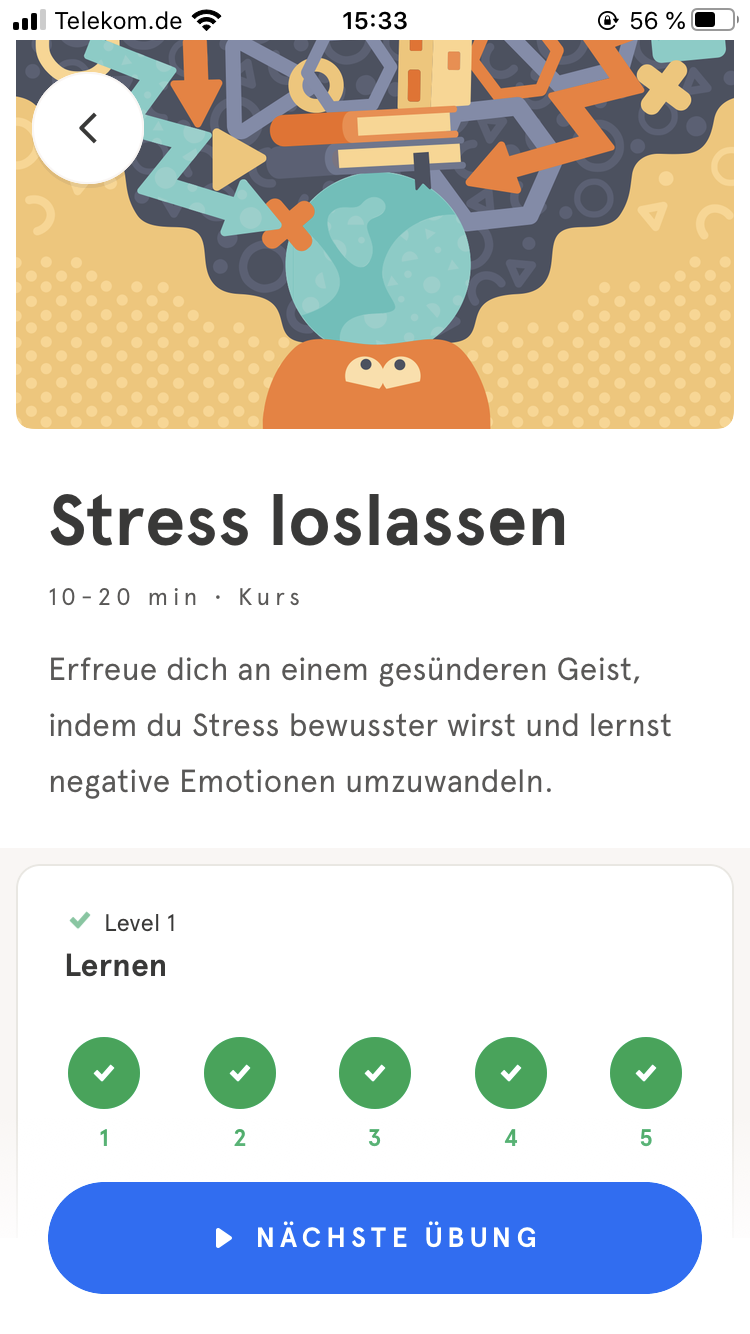
\includegraphics[width=5cm,keepaspectratio]{headspace1}
  \end{minipage}
  \begin{minipage}[t]{0.45\linewidth} 
  \centering 
   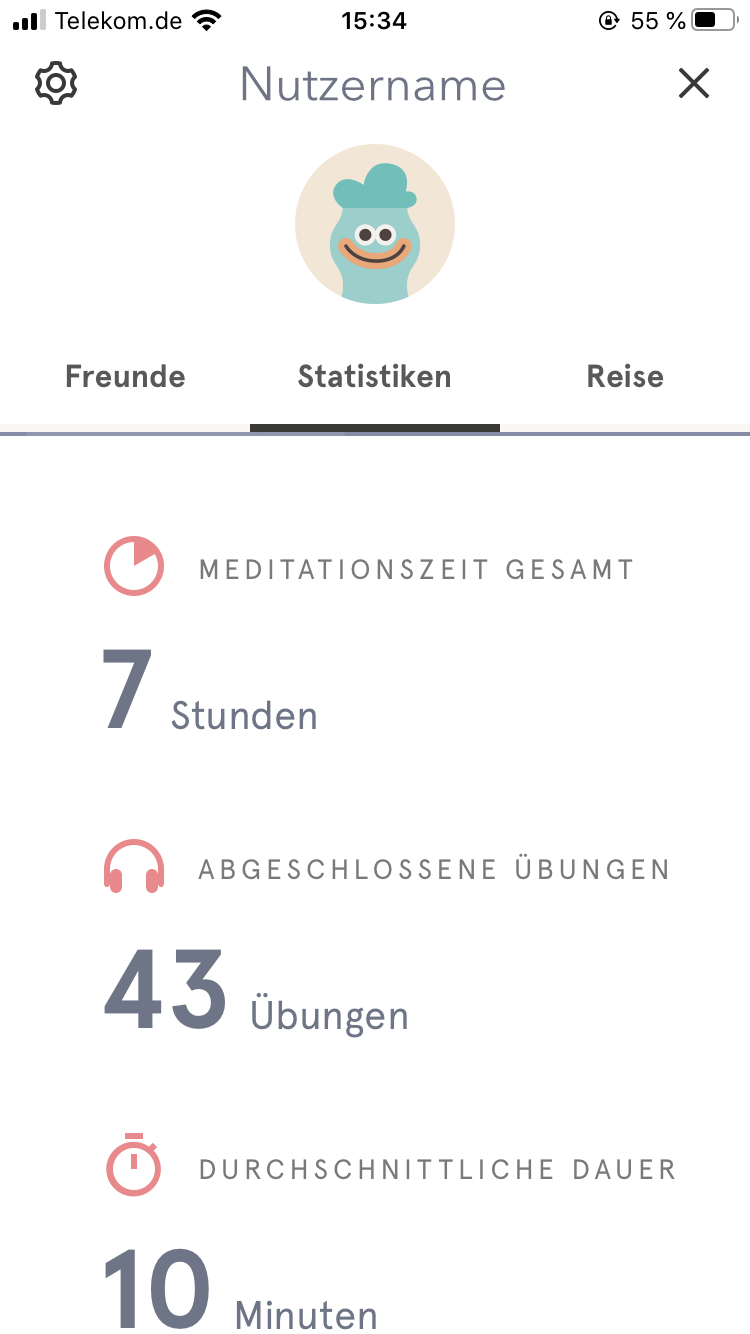
\includegraphics[width=5cm,keepaspectratio]{headspace2}
  \end{minipage}
    \caption{Kurs Stress loslassen \& Nutzerprofil}  der App \textit{Headspace} 
   \label{fig:headspace}
\end{figure}


\subsection{Related Works}
Mehrere Studien belegen die stressreduzierende Wirkung von Mindfulness-Praktiken. So ergab eine Studie aus dem Jahre 2011 (mit rund 300 Probanden die einen achtwöchtigen Mindfulness-Stressmanagementkurs durchliefen), dass derartige Praktiken dazu beitragen können einen Bewusstseinszustand zu trainieren, der eine bessere Interpretation von Stresssituationen und damit auch einen besseren/positiveren Umgang mit diesen zulässt \zit{MindfulnessStudy1}. 

Eine von der TU-Chemnitz durchgeführte Metaanalyse mehrerer  Arbeiten, welche sich mit Mindfulness- und MBSR-Programmen auseinandersetzen, zeigt, dass hinsichtlich psychischer Gesundheit MBSR-Trainings mit Meditationselementen die größte positive Wirkung verzeichnen können \zit{MindfulnessStudy2}.

Aber auch explizit im studentischen Umfeld gibt es bereits verschiedene Forschungen, die sich mit Mindfulness im Bezug auf Stressreduktion beschäftigen. So evaluierten mehrere in Jena ansässige Wissenschaftler, in ihrer Studie aus dem Jahre 2020, die Auswirkungen von MBSR-Programmen auf das physiologische Stressempfinden von Studenten. Hierzu wurden verschiedene Körperfunktionen (z.B. Puls, Blutdruck) der Testpersonen überwacht, während diese an einem achtwöchigen MBSR-Trainingsprogramm, welches eigens für Studenten und deren Lebensumstände angepasst wurde, teilnahmen. Die Interventionsgruppe zeigte im Verlauf des Experiments, verglichen mit der Kontrollgruppe, bessere Ergebniswerte. Damit lässt sich auf ein gesenktes Stressniveau und im weiteren Sinne auf gesundheitlich positive Effekte schließen \zit{MindfulnessStudy3}.

Das Thüringer Modellprojekt mit dem Namen \textit{Achtsame Hochschulen in der digitalen Gesellschaft} forschte bis 2019 zum Thema Achtsamkeit im Hochschulkontext und bezieht neben Stress auch die zunehmende Digitalisierung mit ein. Hierzu wurden verschiedene Praktiken analysiert und evaluiert um anschließend entsprechende Angebote für Studenten und Lehrende zu entwerfen bzw. weiterzuentwickeln. Diese Angebote werden weiterhin sowohl sozialwissenschaftlich, als auch medizinisch objektiv evaluiert um neue Erkenntnisse bezüglich Achtsamkeit, Stressminderung und allgemeinem Wohlbefinden im Hochschulumfeld zu erlangen.  \zit{AchtsameHochschulen}.

Bereits mehrere Studien befassen sich explizit mit \textit{Mindfulness Apps} und deren Effekte auf Studenten hinsichtlich Stressminderung und psychischer Gesundheit im Allgemeinen. So untersuchten US-amerikanische Wissenschaftler 2019 die möglichen Auswirkungen der Smartphone-App \textit{Calm} bei regelmäßiger Nutzung. Hierbei konnten vergleichbare Effekte festgestellt werden, wie bei klassischen MBSR-Kursen bei denen ein persönlicher Kontakt zu einem Trainer/Trainingsgruppe notwendig ist \zit{MindfulnessStudy4}. Zu ähnlichen Ergebnissen kommt auch eine Masterarbeit aus dem Jahr 2019. Diese merkt weiterhin die Vorteile einer solchen App gegenüber klassischen Kursen an. Dazu zähle die sofortige, ortsunabhängige Verfügbarkeit und die damit einhergehende Zeitersparnis genauso wie die Kostenersparnis, beispielsweise durch das Wegfallen eines professionellen Trainers \zit{MindfulnessStudy5}.

\section{METHODIK UND DURCHFÜHRUNG}
Um die Forschungsfrage beantworten zu können wird die Arbeit in zwei Aufgabenbereiche gegliedert, einer Metaanalyse bereits vorhandener Literatur und die Durchführung mehrerer Leitfadeninterviews. 
Eine Metaanalyse im herkömmlichen Sinn, also eine quantitative Kodierung und Auswertung vorhandener Forschung, ist aufgrund des geringen (zeitlichen) Umfangs dieser Arbeit nicht möglich. Vielmehr erfolgt dieser Arbeitsschritt in Annäherung an eine systematische Überssichtsarbeit, um relevante Forschungsarbeiten zusammenzufassen und letztendlich die gegebene Fragestellung besser beantworten zu können \zit{Metaanalyse}.

Die Schlussfolgerungen, die die Auswertungen der bereits bestehenden Quellen und Related Works (siehe Abschnitt 2) zulassen, dienen als Grundlage für die Erstellung bzw. Entwicklung eines Fragebogens für Leitfadeninterviews. Leitfadeninterviews bezeichnen eine qualitative Erhebungs- bzw. Forschungsmethode bei der mehrere Interviews mithilfe eines vorher definierten, mehr oder weniger strukturierten, Fragebogens geführt werden. Für diese Arbeit wurde ein Fragenkatalog erstellt, der je nach Gesprächsverlauf flexibel abgearbeitet werden kann. Kommen während des Interviews weitere, neue Fragen / Antworten auf, sind auch diese zulässig. Bei den Fragen soll es sich hauptsächlich um offene Fragestellungen handeln, um bestmöglich an neue Informationen / Aussagen zu gelangen \zit{Leitfadeninterview}.
Die Auswahl der Gesprächspartner erfolgt hauptsächlich nach dem Kriterium, dass diese in der Zielgruppe, also aktuell Studierende, sein müssen.

Die eigentlichen Interviews werden als Einzelgespräche über einen Audio- bzw. Videoanruf auf den Plattformen \textit{Zoom} bzw. \textit{Discord} geführt und mit Einverständnis des jeweiligen Gegenübers aufgezeichnet. 
Im Nachgang erfolgt das Transkribieren der Gespräche in zwei Schritten. Erst wird die jeweilige Audioaufzeichnung mithilfe der computergestützten Spracheingabe auf der Plattform \textit{Google Docs} zu Text umgewandelt. Im Nachgang erfolgt ein manuelles \grqq Sichten\grqq\ der Aufnahme und gegebenenfalls das Ausbessern von fehlerhaften oder nicht transkribierten Aussagen. 
Sind alle Interviews transkribiert, erfolgt eine qualitative Inhaltsanalyse nach Kuckartz in mehreren Schritten. Zu Beginn werden die vorhandenen Transkripte ausgewertet und erste thematische Hauptgruppen generiert. Auf Grundlage dieser Gruppen werden alle vorliegenden Interviews codiert und die jeweilig gleich codierten Stellen zusammengestellt um daraus induktiv sog. Subkategorien bestimmen zu können. Sind alle Inhalte entsprechend codiert bzw. kategorisiert, kann mit der eigentlichen Auswertung begonnen werden. Hier wird versucht neue Zusammenhänge zwischen verschiedenen Kategorien und bereits bestehendem Wissen zu erkennen, als auch verschiedene Aussagen zusammenzufassen bzw. zu generalisieren. Die Codierung und allgemeine Textarbeit findet ebenfalls computergestützt mit der Software \textit{MAXQDA2020} statt. Im Nachgang erfolgt dann die Ergebnispräsentation \zit{Inhaltsanalyse}. Aufgrund des begrenzten Umfangs und des zeitlichen Rahmens wird auf eine Reliabilitätsprüfung dieser Arbeit verzichtet.

\subsubsection{Interview Durchführung}
Für die Durchführung der Interviews wurde mit jedem Befragten ein individueller Termin vereinbart, zu dem sich dann auf der vorher bestimmten Online-Plattform getroffen wurde. Nach einer Begrüßung wurde der Befragte kurz darüber informiert, dass es sich bei dem Interview grob um das Thema  \grqq Stress\grqq\ handle. Weiterhin, dass das Gespräch aufgezeichnet und später transkribiert wird, um es für die Arbeit auswerten zu können. Bevor die eigentlichen Fragen gestellt wurden, wurde das Gegenüber darüber aufgeklärt, dass die Befragung anonym verarbeitet wird, Fragen ehrlich und ausführlich beantwortet werden sollen und bei Fragen die nicht beantwortet werden möchten dies kommuniziert und keine Falschaussage getroffen werden soll. Im Anschluss an das Interview wurde sich bei der befragten Person für die aufgebrachte Zeit bedankt und gegebenenfalls weitere Informationen über die Arbeit bzw. das Ziel der Arbeit gegeben.
Insgesamt wurden 6 Interviews durchgeführt, wovon alle Gesprächspartner (drei weibliche, drei männliche Personen) aktuell eingeschriebene Studenten an einer bayrischen Hochschule oder Universität sind. 

\subsubsection{Fragenkatalog}
Der Fragenkatalog für die Leitfadeninterviews kann in verschiedene Kategorien untergliedert werden, die sich vorab durch Analyse bestehender Quellen (siehe Abschnitt 2) ergaben. Diese teilen sich auf in: 
\begin{itemize}[itemsep=0.5mm, parsep=0pt]
\item  Allgemeine Informationen \textit{A}
\item  Stress \& Stressempfinden \textit{B}
\item  Stressbewältigung \& Stressvorbeugung \textit{C}
\item  Smartphone-Nutzung \textit{D}
\item  Achtsamkeit \& Meditation \textit{E}
\item  Fragen, falls schon eine Mindfulness-App genutzt wird \textit{F}
\end{itemize}

Insgesamt enthält der Katalog rund 30 Fragen, davon sind ca. vier bis fünf Fragen als geschlossene Fragen anzusehen (z.B. \textit{Wie ist dein Geschlecht?}). Je nach Interviewverlauf können neue, sich aus dem Gespräch ergebene, Fragen zusätzlich gestellt werden oder eine Frage aus dem Katalog weggelassen werden, wenn eine vorherige Antwort diese ausschließt bzw. irrelevant macht.


\begin{longtable}{|>{\hspace{0pt}}p{0.273\linewidth}|>{\hspace{0pt}}p{0.668\linewidth}|} 
\hline
Kategorie & Fragestellung \\* 
\hline
\multirow{2}{0.273\linewidth}{\hspace{0pt}\textit{A}} & {\cellcolor[rgb]{0.949,0.949,0.949}}\textit{A1}~Wie alt bist du? \\* 
\cline{2-2}
 & \textit{A2}~Erzähle mir doch etwas zu deinem Studium \\* 
\hline
\multirow{4}{0.273\linewidth}{\hspace{0pt}\textit{B}} & {\cellcolor[rgb]{0.949,0.949,0.949}}\textit{B1}~In welchen Lebensbereichen empfindest du Stress? \\* 
\cline{2-2}
 & \textit{B2}~Wie würdest du die Arbeits-/Zeitbelastung durch dein Studium einschätzen? \\* 
\hhline{|~-|}
 & {\cellcolor[rgb]{0.949,0.949,0.949}}\textit{B3}~Was ist Stress für dich? / Was verstehst du unter Stress? \\* 
\cline{2-2}
 & \textit{B4}~Woran machst du fest, dass du gestresst bist? \\* 
\hline
\multirow{5}{0.273\linewidth}{\hspace{0pt}\textit{C}} & {\cellcolor[rgb]{0.949,0.949,0.949}}\textit{C1}~Wie gehst du damit um, wenn du mehrere Aufgaben (z.B. für Uni oder Arbeit) gleichzeitig zu erledigen/abzugeben hast? \\* 
\cline{2-2}
 & \textit{C2}~Was sind deiner Meinung nach Dinge, die man vorbeugend tun kann, um Stress zu vermeiden? \\* 
\hhline{|~-|}
 & {\cellcolor[rgb]{0.949,0.949,0.949}}\textit{C3}~Kennst du längere Stressphasen, wenn ja welche? \\* 
\cline{2-2}
 & \textit{C4~}Wie gehst du mit einer längeren Stressphase (z.B. Klausurenphase) um, hast du bestimmte Strategien die dir dabei helfen? \\* 
\hhline{|~-|}
 & {\cellcolor[rgb]{0.949,0.949,0.949}}\textit{C5}~Wie sieht Entspannung / Entspannungsphasen für dich konkret aus? \\* 
\hline
\multirow{3}{0.273\linewidth}{\hspace{0pt}\textit{D}} & \textit{D1}~Nutzt du Gesundheits-/Healthapps (z.B. Trainingsapps, Tracker)? \\* 
\hhline{|~-|}
 & {\cellcolor[rgb]{0.949,0.949,0.949}}\textit{D2}~Welche nennenswelchen Features haben diese Apps? \\* 
\cline{2-2}
 & \textit{D3}~Denkst du eine App könnte dir beim Entspannen helfen? Welche Features müsste diese haben? \\* 
\hline
\multirow{4}{0.273\linewidth}{\hspace{0pt}\textit{E}} & {\cellcolor[rgb]{0.949,0.949,0.949}}\textit{E1}~Hast du dich schon mal Entspannungsübungen (z.B. Atemübungen, Meditation) ausprobiert? \\* 
\cline{2-2}
 & \textit{E2}~Was denkst du, denkt die Gesellschaft über Dinge wie Achtsamkeits- oder Meditationsübungen? \\* 
\hhline{|~-|}
 & {\cellcolor[rgb]{0.949,0.949,0.949}}\textit{E3}~Was denkst du persönlich darüber? \\* 
\cline{2-2}
 & \textit{E4}~Was müsste dir eine App bieten, dass du sie regelmäßig für diesen Zweck nutzt? \\* 
\hline
\multirow{3}{0.273\linewidth}{\hspace{0pt}\textit{F}} & {\cellcolor[rgb]{0.949,0.949,0.949}}F1 Was versprichst du dir von dieser App? \\* 
\cline{2-2}
 & \textit{F2}~Wieso nutzt du genau diese App? \\* 
\hhline{|~-|}
 & {\cellcolor[rgb]{0.949,0.949,0.949}}\textit{F3}~Wie bist du zu der App gekommen? \\
\hline
\caption{Auszug aus dem Fragenkatalog}
\label{table:fragen}
\end{longtable}

Die Fragen der Kategorie \textit{A} sollen grundlegende Informationen klären und in das Gespräch einführen. Folgend soll in der zweiten Kategorie (\textit{B}) herausgefunden werden, ob überhaupt und wie der Befragte, im Kontext des Studiums, Stress empfindet und wie er Stress definiert. Die Fragen des Abschnittes \textit{C} dienen der Feststellung von bereits vorhandenen Stress-Bewältigungsstrategien und der Hinführung zum Thema Entspannung. Mit den \textit{D} Fragen soll kurz leicht Abstand vom eigentlichen Thema genommen werden. Die Antworten sollen des weiteren erste Aufschlüsse darüber geben, wie der Befragte eine solche  \grqq Mindfulness App\grqq\ annehmen würde. Die Kategorie \textit{E} befasst sich hauptsächlich mit Akzeptanz und Interesse des Gegenübers hinsichtlich Entspannungs- und Meditationsübungen. Nutzt der Gesprächspartner bereits eine \grqq Mindfulness App\grqq\ , so sollen die Fragen \textit{F} klären weshalb und wie die App jeweils verwendet wird.

\section{AUSWERTUNG}
Folgend werden die aus den Leitfadeninterviews gewonnenen Informationen mit den theoretischen Grundlagen und vorausgegangenen Forschungen (siehe Abschnitt 2) in Zusammenhang gebracht. So können zusammenfassende Thesen generiert werden, welche beispielhaft mit Ankersätzen aus den geführten Gesprächen gestützt werden. Die Untergliederung orientiert sich an vorher gebildeten Codierungen bzw. Kategorien, denen passende Textpassagen aus den Transkripten zugeordnet wurden.

\subsection{Stress im Studium}

\subsection{Stressbewältigung}
\subsection{Einstellung gegenüber Mindfulness-Praktiken}
\subsection{Positive Effekte der Nutzung}
\subsection{Begünstigende Faktoren für die Nutzung}

\section{FAZIT}
Das Ziel dieser Arbeit war  es in erster Linie zu evaluieren ob und wie sogenannte \grqq Mindfulness Apps\grqq\ zur Stressbewältigung im Alltag eines Studenten beitragen können. 
Neben der Bestätigung, dass derartige Anwendungen in gewissem Umfang tatsächlich positive Auswirkungen auf den Umgang mit Stress haben können, konnte auch festgestellt werden, welche Kriterien und Voraussetzungen zu einer...... XXXX

Allerdings ist zu beachten, dass es sich bei dieser Arbeit lediglich um eine Seminararbeit handelt, welche hinsichtlich des Umfangs deutlich geringer ausfällt, als beispielsweise eine Masterarbeit und dementsprechend eher als Grundlagenforschung anzusehen ist. 

Kritisiert werden sollten auch die eher geringe Anzahl Gesprächspartner und die teils zu wenig theoriebasierten  Fragestellungen. Mit mehr Probanden aus unterschiedlicheren sozialen Gruppen (also nicht nur in Würzburg ansässige Studenten) ließen sich gegebenenfalls vielseitigere Antworten generieren. Fragestellungen, welche teils noch näher an wissenschaftliche Theorien und vorausgegangene Forschungen angelehnt wären, würden eine bessere Überprüfbarkeit der Forschungsergebnisse erlauben. Des Weiteren ist zu beachten, dass auf eine Reliabilitätsprüfung verzichtet wurde.

Nichtsdestotrotz weißen die, hauptsächlich aus den Interviews generierten, Hypothesen große Übereinstimmungen mit den Ergebnissen vorangegangener Forschungen im gleichen Themenumfeld auf und untermauern diese.

Es ist zu empfehlen weitere Studien hinsichtlich dieser Thematik anzustellen. So können Forschungen, die die tatsächliche Nutzung einer solchen App und deren Auswirkungen (psychisch, physisch) über einen gewissen Zeitraum untersuchen (also beispielsweise mit studentischen Probanden) womöglich von großem Erkenntnisgewinn sein. Weiterhin könnten damit vorangegangene Forschungen, wie diese, mit objektiven Fakten, wie z.B. Messwerten, bestätigt werden.


\nocite{*}
\printbibliography

\end{document}